\section{Übersetzungs-Phasen}


\begin{frame}{Übersetzungs-Phasen (phases of translation)}
	Der Code durchläuft im Wesentlichen drei Arbeitsschritte:
	
	\begin{enumerate}
		\item Präprozessor
		\item Compiler
		\item Linker
	\end{enumerate}
\end{frame}

\begin{frame}[fragile]{Übersetzungs-Phasen}
	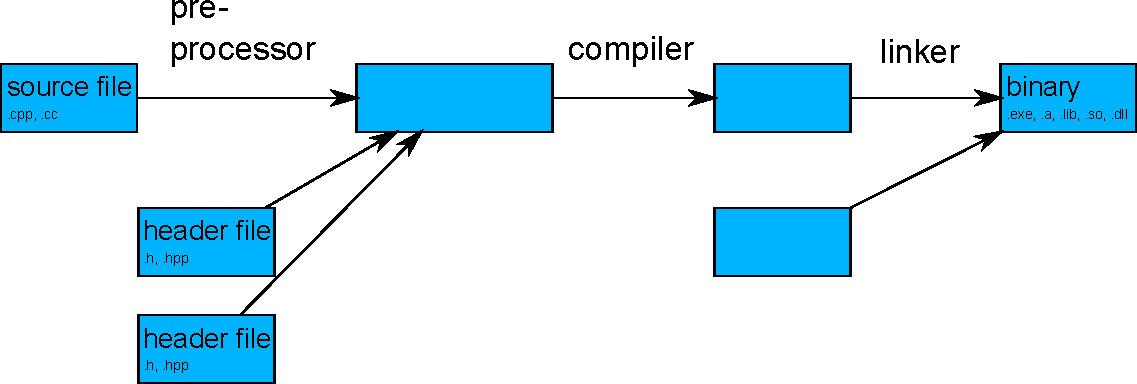
\includegraphics[width=\textwidth]{images/translation-simple}
\end{frame}

\subsection{Der Präprozessor}

\begin{frame}[fragile]{Präprozessor}
	Der Präprozessor ersetzt Teile des Quelltexts nach bestimmten Regeln.
	
	\vspace{2em}
	
	\begin{itemize}
		\item Einfügen von Dateiinhalten \verb|#include| \\
		      (der Präprozessor wird auch für die eingefügte Datei ausgeführt!)
		\item Suchen \& Ersetzen \verb|#define|
		\item Bedingtes Einfügen \verb|#if|
		\item Abbrechen der Übersetzung \verb|#error|
	\end{itemize}
\end{frame}

\begin{frame}{Präprozessor}
	\begin{block}{Warum?}
		\begin{itemize}
			\item Aufteilung des Projekts auf mehrere Dateien
			\item Verschiedene Build-Konfigurationen (z.B. Debug/Release)
			\item Unterschiedlicher Code für unterschiedliche Plattformen
			\item Automatische Codeerzeugung
			\item ...
		\end{itemize}
	\end{block}
\end{frame}

\begin{frame}[fragile]{Zusammenhang mit der Übersetzung}
	\begin{itemize}
		\item Der Präprozessor wird durch Direktiven (Anweisungen) innerhalb des Quellcodes programmiert.
		\item Präprozessor-Direktiven stehen in einer eigenen Zeile und beginnen mit einem \verb|#|
		\item Die Quellcode-Dateien dienen zugleich als Eingabe für den Präprozessor. Die Ausgabe geht dann in die nächste Übersetzungsphase.
		\item Nach Präprozessor-Direktiven steht \emph{kein} Semikolon \verb|;|
	\end{itemize}
	
	\pause
	\vspace{1em}
	
 	Zeilen, die nicht von Präprozessor-Direktiven betroffen sind, werden vom Präprozessor unverändert ausgegeben.
\end{frame}

\begin{frame}[fragile]{Die include-Direktive}
	\begin{block}{include-Direktive}
		\verb|#include "|\emph{dateiname}\verb|"| \\
		\vspace{0.5em}
		Ersetzt diese Zeile durch den Inhalt der Datei \emph{dateiname}. \\
		Der Inhalt der Datei wird ebenfalls vom Präprozessor verarbeitet.
	\end{block}
	
	\pause
	\vspace{1em}
	
	\small
	Es gibt noch die Variante \verb|#include <|\emph{dateiname}\verb|>|.
\end{frame}

\begin{frame}[fragile]{Die include-Direktive}
	Gängige Compiler unterscheiden zwischen beiden Varianten folgendermaßen:
	\begin{itemize}
		\item Die \verb|"|-Variante ist für Dateien des eigenen Projekts.
		      Der angegebene Pfad wird relativ zum Pfad der aktuellen Datei interpretiert.
		\item Die \verb|<>|-Variante ist für Dateien aus fremden Bibliotheken.
		      Sie werden an vorher festgelegten Orten gesucht. (z.B. für die Std-Lib, boost, Qt usw.)
	\end{itemize}
\end{frame}

\begin{frame}{Beispiel: include}
	\footnotesize
	
	
	\begin{columns}[t]
		\only<1>{
			\column{0.4\textwidth}
			{\normalsize \emph{myheader.h} }
			\vspace{0.5em}
			\lstinputlisting[language=C++, linerange={1-4}]{cpp-code/include-directive.cpp}
		
			\column{0.4\textwidth}
			{\normalsize \emph{main.cpp} }
			\vspace{0.5em}
			\lstinputlisting[language=C++, linerange={7-12}]{cpp-code/include-directive.cpp}
		}
		
		\only<2>{
			\column{0.4\textwidth}
			{\normalsize \emph{Ergebnis} }
			\vspace{0.5em}
			\lstinputlisting[language=C++, linerange={15-23}]{cpp-code/include-directive.cpp}
		}
	\end{columns}
\end{frame}

\begin{frame}[fragile]{Die define-Direktive}
	\begin{block}{define-Direktive}
		\verb|#define NAME TOKEN0 TOKEN1.....| \\
		\vspace{0.5em}
		Definiert ein Makro mit dem Namen \verb|NAME|, die darauf folgenden Token sind optional. Trifft der Präprozessor nach der Definition eines Macros auf das Token \verb|NAME|, so ersetzt er es durch die Token \verb|TOKEN0 TOKEN1....|.
	\end{block}
\end{frame}

\begin{frame}{Beispiel: define-Direktive}
	\footnotesize
	\lstinputlisting[language=C++]{cpp-code/define-directive.cpp}
\end{frame}

\begin{frame}[fragile]{Die define-Direktive}
	Makros können auch Parameter haben (function-like macro):
	\vspace{1em}
	
	\footnotesize
	\alt<2->
	{% on slide 2
		\lstinputlisting[language=C++, linerange=13]{cpp-code/define-parameters.cpp}
	}{% on slide 1
		\lstinputlisting[language=C++, linerange={1-12}]{cpp-code/define-parameters.cpp}
	}
	
	\alert{ACHTUNG! Reine Textersetzung!}
\end{frame}

\begin{frame}[fragile]{Die define-Direktive}
	Wann benutze ich Makros bzw. \verb|#define|?
	
	\vspace{2em}
	\uncover<2->
	{
		\alert{So selten wie möglich!}
		
		Stattdessen lieber typedef, Konstanten, Funktionen, etc.
	}
\end{frame}

\begin{frame}[fragile]{Bedingtes Einfügen}
	\begin{block}{if-, else- und endif-Direktiven}
		\begin{lstlisting}[language=C++]
			#if constant_expression_0
			function_variation1();
			#else
			function_variation2();
			some_other_function();
			#endif
		\end{lstlisting}
		Abhängig vom Wert von \verb|constant_expression_0| wird entweder der Code zwischen \verb|#if| und \verb|#else| oder zwischen \verb|#else| und \verb|#endif| eingefügt.
	\end{block}
\end{frame}

\begin{frame}[t]{Beispiel: Bedingtes Einfügen}
	\footnotesize
	\only<1>{
		\lstinputlisting[language=C++, linerange={1-6}]{cpp-code/conditional-inclusion.cpp}
	}
	\only<2>{
		\lstinputlisting[language=C++, linerange={9-14}]{cpp-code/conditional-inclusion.cpp}
	}
	\only<3>{
		\lstinputlisting[language=C++, linerange={17-28}]{cpp-code/conditional-inclusion.cpp}
	}
\end{frame}


\subsection{Der Compiler}
\begin{frame}[fragile]{Der Compiler}
	Übersetzt von Quellcode in Maschinensprache.
	
	\vspace{1em}
	
	Alles was wir in vorigen Workshops behandelt haben, beschreibt gültige Eingaben für den Compiler (Quellcode).
	
	\vspace{2em}
	
	{\footnotesize (Da C++ kompliziert ist, ist es weder einfach noch hilfreich, eine Übersicht über das zu geben, wie seine Eingabe und Ausgabe zusammenhängt.) }
\end{frame}


\subsection{Der Linker}

\begin{frame}[fragile]{Die translation unit}
	Bisher wurden sowohl vom Präprozessor als auch vom Compiler alle .cpp Dateien getrennt voneinander behandelt.
	
	Der Präprozessor arbeite nun auf einer .cpp-Datei. Er fügt dann Weiteres ein bzw. ersetzt (\verb|#include|, \verb|#define|) und lässt manches aus (\verb|#if|, \verb|#else|).
	
	\vspace{1em}
	
	\begin{block}{translation unit}
		Die Ausgabe des Präprozessors ist dann also die source file (.cpp) plus alle eingebundenen Dateien abzüglich den Auslassungen und mit den Macro-Ersetzungen.\\
		Das Entstandene nennt man \emph{translation unit}.
	\end{block}
\end{frame}

\begin{frame}[fragile]{Übersetzungs-Phasen}
	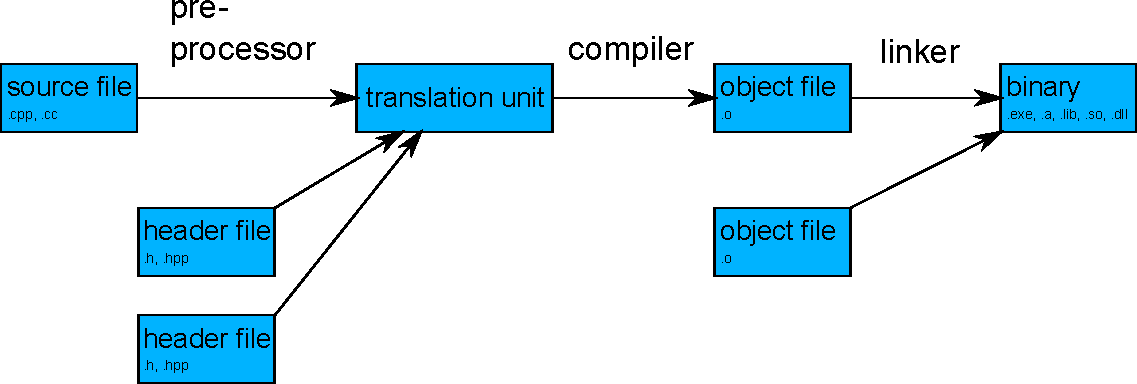
\includegraphics[width=\textwidth]{images/translation}
\end{frame}

\begin{frame}{Linkage}
	Eine translation unit wird dann vom Compiler tatsächlich \emph{übersetzt}, also kompiliert. Es werden alle translation units des Projektes übersetzt und anschließend verknüpft (gelinkt).
	
	\vspace{1em}
	
	\begin{block}{linkage (Standard, 3.5:2)}
		Hat in einer translation unit der Name eines »Dinges«, Referenz, Funktion, Typ, template oder namespace \emph{external linkage}, so darf auf das Etwas, das der Name benennt, auch in anderen translation units zugegriffen werden.
	\end{block}
	Im Normalfall hat ein Name in einem namespace (also nicht innerhalb einer Klassen oder Funktion) external linkage.
	
	\vspace{1em}
	\pause
	
	Aber: Da zuvor schon kompiliert wird, muss dem Compiler gesagt werden, dass dieses Etwas überhaupt existiert.\\
	\tiny
	Siehe: \url{https://github.com/downloads/kit-cpp-workshop/workshop-ss12-03/addendum-header.pdf}
\end{frame}

\begin{frame}{Beispiel: external linkage}
	\footnotesize
	\begin{columns}[t]
		\column{0.4\textwidth}
		translation unit \emph{square.cpp}
		\vspace{1em}
		\lstinputlisting[language=C++, linerange={1-4}]{cpp-code/linkage.cpp}
		
		\pause
		
		\column{0.4\textwidth}
		translation unit \emph{main.cpp}
		\vspace{1em}
		\lstinputlisting[language=C++, linerange={7-12}]{cpp-code/linkage.cpp}
	\end{columns}
\end{frame}

\begin{frame}{Klassen und Linkage}
	member functions von Klassen (Methoden) sind auch nur Funktionen, d.h. sie dürfen auch in anderen translation units verwendet werden.
	
	Dem Namen einer Klassen selbst schreibt man auch linkage zu. Hat der Name einer Klasse external linkage, so bedeutet dies nur, dass die Namen der member functions external linkage haben.
	
	\pause
	\vspace{1em}
	
	\footnotesize
	\begin{columns}[t]
		\column{0.4\textwidth}
		translation unit \emph{square.cpp}
		\vspace{1em}
		\lstinputlisting[language=C++, linerange={15-23}]{cpp-code/linkage.cpp}
		
		\pause
		\column{0.4\textwidth}
		translation unit \emph{main.cpp}
		\vspace{1em}
		\lstinputlisting[language=C++, linerange={15-18, 25-30}]{cpp-code/linkage.cpp}
	\end{columns}
\end{frame}

\begin{frame}[fragile]{Linkage-Modifier}
	Im Normalfall hat ein Name in einem namespace (also nicht innerhalb einer Klassen oder Funktion) external linkage.
	
	\vspace{1em}
	
	Man kann die Linkage durch die Schlüsselwörter \verb|extern| und \verb|static| sowie durch unbenannte namespaces beeinflussen:
	
	\pause
	
	\begin{block}{static im Bezug auf Linkage}
		Schreibt man vor die Definition eines »Dinges«, einer Referenz oder einer Funktion \verb|static|, so hat der Name \emph{internal linkage}.
	\end{block}
	
	\pause
	
	\begin{block}{unnamed namespaces}
		Alles innerhalb eines unbenannten namespaces \verb|namespace { /*...*/ }| hat erst einmal \emph{internal linkage}. Dies \enquote{vererbt} sich bspw. auf alle darinnen deklarierten Funktionen.
	\end{block}
\end{frame}

\begin{frame}{Beispiel: Linkage-Modifier}
	\footnotesize
	\alt<2>
	{% on slide 1
		\lstinputlisting[language=C++, tabsize=4]{cpp-code/linkage-modifiers.cpp}
	}{% on slide 2
		\lstinputlisting[language=C++, tabsize=4, commentstyle=\none]{cpp-code/linkage-modifiers.cpp}
	}
\end{frame}
